\documentclass[obeyspaces]{beamer}
\usetheme{bjeldbak}
\usepackage{ragged2e}
\newcommand{\columnsbegin}{\begin{columns}}
\newcommand{\columnsend}{\end{columns}}
\setbeamertemplate{caption}[numbered]
\setbeamertemplate{caption label separator}{:}
\setbeamercolor{caption name}{fg=normal text.fg}
\usepackage{amssymb,amsmath,fancyvrb}
\usepackage{ifxetex,ifluatex}
\usepackage{fixltx2e} % provides \textsubscript
\usepackage{lmodern}
\ifxetex
  \usepackage{fontspec,xltxtra,xunicode}
  \defaultfontfeatures{Mapping=tex-text,Scale=MatchLowercase}
  \newcommand{\euro}{€}
\else
  \ifluatex
    \usepackage{fontspec}
    \defaultfontfeatures{Mapping=tex-text,Scale=MatchLowercase}
    \newcommand{\euro}{€}
  \else
    \usepackage[T1]{fontenc}
    \usepackage[utf8]{inputenc}
      \fi
\fi
% use upquote if available, for straight quotes in verbatim environments
\IfFileExists{upquote.sty}{\usepackage{upquote}}{}
% use microtype if available
\IfFileExists{microtype.sty}{\usepackage{microtype}}{}
\usepackage{longtable,booktabs}
\usepackage{caption}
% These lines are needed to make table captions work with longtable:
\makeatletter
\def\fnum@table{\tablename~\thetable}
\makeatother

%\usepackage{hyperref}
\def\UrlBreaks{\do\/\do-}

\usepackage{bm}

% Comment these out if you don't want a slide with just the
% part/section/subsection/subsubsection title:
% \AtBeginPart{
%   \let\insertpartnumber\relax
%   \let\partname\relax
%   \frame{\partpage}
% }
% \AtBeginSection{
%   \let\insertsectionnumber\relax
%   \let\sectionname\relax
%   \frame{\sectionpage}
% }
% \AtBeginSubsection{
%   \let\insertsubsectionnumber\relax
%   \let\subsectionname\relax
%   \frame{\subsectionpage}
% }
\usepackage{tikz}
\usetikzlibrary{decorations.pathreplacing,calc}
\newcommand{\tikzmark}[1]{\tikz[overlay,remember picture] \node (#1) {};}

\setbeamersize{text margin left=2em,text margin right=2em}



\setlength{\parindent}{0pt}
\setlength{\parskip}{6pt plus 2pt minus 1pt}
\setlength{\emergencystretch}{3em}  % prevent overfull lines
\setcounter{secnumdepth}{0}
\providecommand{\tightlist}{%
  \setlength{\itemsep}{0pt}\setlength{\parskip}{0pt}}

\DeclareMathOperator*{\argmin}{arg\,min}

\newcommand{\twopartdef}[4]
{
  \left\{
    \begin{array}{ll}
      #1 & \mbox{if } #2 \\
      #3 & \mbox{if } #4
    \end{array}
  \right.
}

\newcommand{\twopartdefo}[3]
{
  \left\{
    \begin{array}{ll}
      #1 & \mbox{if } #2 \\
      #3 & \mbox{otherwise}
    \end{array}
  \right.
}

%gets rid of bottom navigation bars
\setbeamertemplate{footline}[frame number]{}

%gets rid of navigation symbols
\setbeamertemplate{navigation symbols}{}

\DeclareMathOperator*{\argmax}{arg\,max}


\newcommand{\vect}[1]{\boldsymbol{#1}} % Uncomment for BOLD vectors.

\title{Recommender Systems}
\author{Spyros Samothrakis\\
 Research Fellow, IADS\\
 University of Essex}
\date{February 14, 2017}

\begin{document}
\frame{\titlepage}

\begin{frame}
\tableofcontents[hideallsubsections]
\end{frame}

\section{About}\label{about}

\begin{frame}{Recommmender Systems}

\begin{itemize}
\tightlist
\item
  We will discuss one of the most popular applications of data science

  \begin{itemize}
  \tightlist
  \item
    Recommender Systems
  \end{itemize}
\item
  Every website does it, either in the context of e-mail or in the
  context of
\item
  Recommender Systems match users with items
\item
  Users under constant information overload
\item
  Think songs, foods, drinks, movies
\end{itemize}

\end{frame}

\begin{frame}{Examples}

\begin{itemize}
\tightlist
\item
  Proposing food, songs
\item
  Proposing books
\item
  Proposing friends
\item
  This is even done offline in the service industry!
\item
  Can you think of other examples?
\end{itemize}

\end{frame}

\section{RS as a supervised learning
problem}\label{rs-as-a-supervised-learning-problem}

\begin{frame}{Content-based filtering}

\begin{itemize}
\tightlist
\item
  User
\end{itemize}

\end{frame}

\begin{frame}{Demographic}

\end{frame}

\begin{frame}{}

\end{frame}

\begin{frame}{Knowledge based}

\end{frame}

\section{RS as a contextual bandit
problem}\label{rs-as-a-contextual-bandit-problem}

\section{RS as collaborative
filtering}\label{rs-as-collaborative-filtering}

\begin{frame}{Collaborative filtering}

\begin{itemize}
\tightlist
\item
  Collaborative filtering is an effort to predict how products/items
  will be rated by a user, given previous ratings (from both the user
  and others)
\item
  This prediction can help us recommend to the user only items that we
  think she will rate highly
\item
  Latent Factor Models - Netflix Challenge (1M\(\$\))- Simon Funk
\end{itemize}

\end{frame}

\begin{frame}{Same sample data}

\center

\tiny

\begin{tabular}{lrrrrr}    
\toprule
{} &  \textbf{The Call of Cthulhu} &   \bf Frankenstein &   \bf Dracula &   \bf Neuromancer & \bf  Dune \\
\midrule
\bf 0 &                    6 &              0 &         0 &             7 &             NaN \\
\bf 1 &                    5 &              0 &         5 &             6 &               5 \\
\bf 2 &                    9 &            NaN &         4 &           NaN &               8 \\
\bf 3 &                    4 &            NaN &         2 &             5 &               6 \\
\bf 4 &                    4 &            NaN &         4 &             6 &               0 \\
\bf 5 &                    6 &              3 &         8 &             5 &               7 \\
\bf 6 &                  NaN &              6 &       NaN &             6 &               7 \\
\bf 7 &                  NaN &              1 &         1 &             6 &             NaN \\
\bf 8 &                  NaN &            NaN &         2 &           NaN &               9 \\
\bf 9 &                  NaN &              3 &         4 &             5 &               7 \\
\bottomrule
\end{tabular}

\end{frame}

\begin{frame}{Factors}

\begin{itemize}
\tightlist
\item
  We are going to base our predictions on ``hidden'' qualities of the
  items
\item
  For example, food can have different levels of spiciness, a drink
  different levels of bitterness
\item
  We term these qualities ``factors''
\item
  A more sensible way of describing items would be to see them as a
  collection of ``factors''

  \begin{itemize}
  \tightlist
  \item
    But our data is just ratings!
  \end{itemize}
\item
  Thus, our factors are ``Latent'', i.e.~hidden!
\end{itemize}

\end{frame}

\begin{frame}{Example Factors for our data}

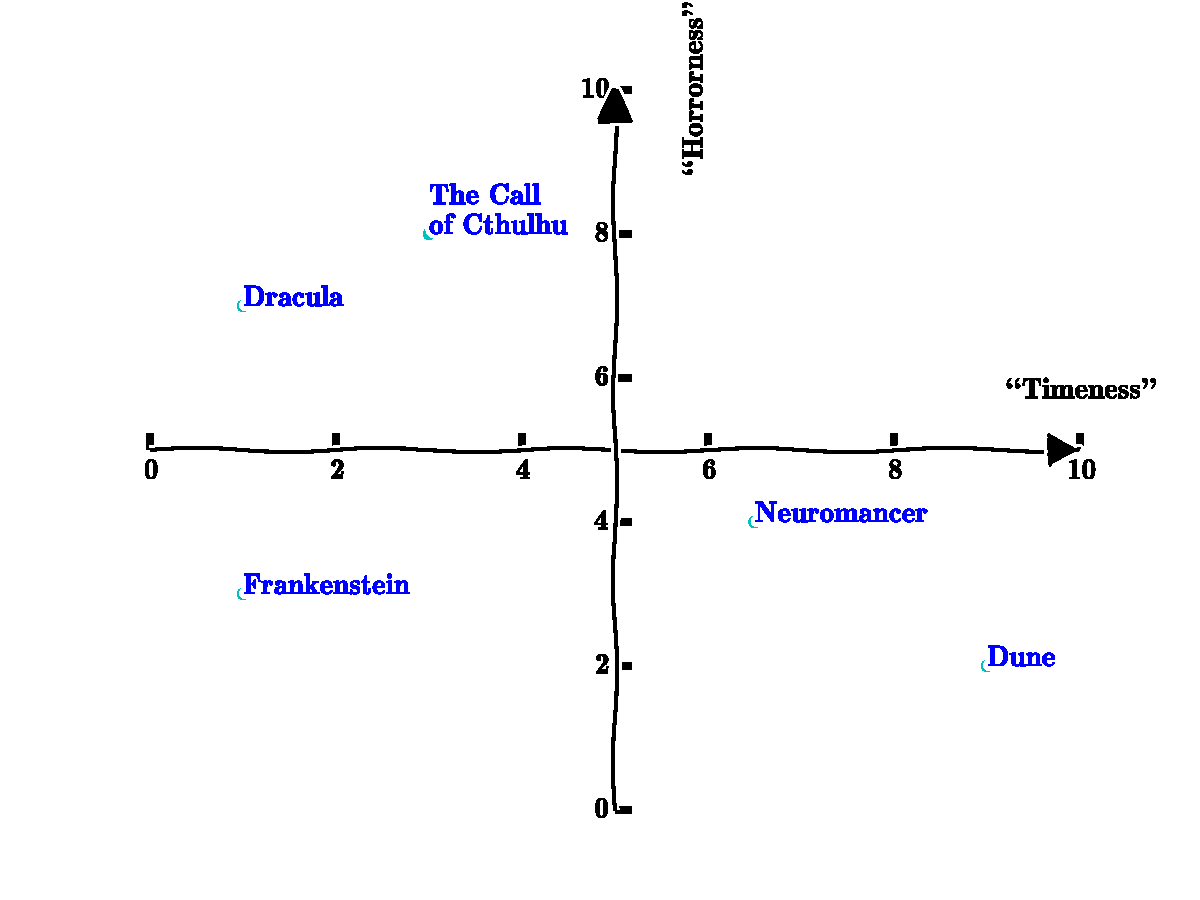
\includegraphics[width=\textwidth]{./graphics/lec5/books.pdf}

\end{frame}

\begin{frame}{Factors and User Preferences}

\begin{itemize}
\tightlist
\item
  Let's assume \(n\) factors
\item
  We can encode factors as a real valued vector
  \(\vect{\mathit{item\_factors}_i}= [\phi_0, \phi_1, ... , \phi_{n-1}]\)
\item
  For example ``The Call of the Cthulhu'' can be encoded as
  \(\vect{\mathit{item\_factors}_{0}} = [3,8]\)
\item
  Each user now can have preferences over factors, encoded as weights
  \(\vect{\mathit{user\_preferences}_j} = [w_0, w_1, ... , w_{n-1}]\)
\item
  The weight vector contains user preferences, e.g.
  \(\vect{user\_preferences_{0}} = [0.5,0.8]\)
\item
  But we don't have any user weights nor any item factors - generate
  some random!
\end{itemize}

\end{frame}

\begin{frame}{Some random data}

\begin{itemize}
\tightlist
\item
  Each row in \(\vect{user\_preferences}\) represents the preferences of
  a user, while each row in \(\vect{item\_factors}\) represents the
  factors of an item
\end{itemize}

\begin{Verbatim}[fontsize=\scriptsize]

array([[ 0.092,  0.783],          array([[ 0.338,  0.519],   
       [ 0.78 ,  0.488],                 [ 0.69 ,  0.256],
       [ 0.844,  0.062],                 [ 0.363,  0.93],            
       [ 0.68 ,  0.549],                 [ 0.004,  0.112],       
       [ 0.212,  0.43 ],                 [ 0.608,  0.104]])  
       [ 0.961,  0.023],
       [ 0.659,  0.31 ],
       [ 0.92 ,  0.769],
       [ 0.817,  0.452],
       [ 0.834,  0.887]])

\end{Verbatim}

\(rating[0][0] \gets 0.437 = 0.092 * 0.338 + 0.783* 0.519\)

Far away from the observed rating of \(6\)

\end{frame}

\end{document}
